%% using aastex version 6.2
\documentclass[twocolumn, dvipdfmx]{aastex62}
\usepackage{CJK}
\usepackage{textcomp}
\usepackage{graphicx}
\usepackage{here}
\usepackage{hhline}
\usepackage{longtable}

\newcommand\aastex{AAS\TeX}
\newcommand\latex{La\TeX}

\received{\today}
\revised{\today}
\accepted{\today}
\submitjournal{ApJ}

\shortauthors{Goda \& Matsuo}

\begin{document}
\begin{CJK*}{UTF8}{min}

\title{Multiple populations of extrasolar gas giants}

\author{Shohei Goda}
\affil{\rm Department of Earth and Space Science, Graduate School of Science, Osaka University, 1-1, Machikaneyamacho, Toyonaka, Osaka 560-0043, Japan}

\author{Taro Matsuo}
\affiliation{\rm Department of Earth and Space Science, Graduate School of Science, Osaka University, 1-1, Machikaneyamacho, Toyonaka, Osaka 560-0043, Japan}


\begin{abstract}

Statistically verifying the character of exoplanets, we can expect to reveal the formation or evolution processes of planetary systems. The notable parameters of planetary systems are metallicity of host star, planet mass, and eccentricity. Gas giants around metal rich stars are easily formed by core accretion. Since these planets are grown with bottom up, the distributions of planet masses and eccentricities are seemed to be continuously extended.
On the other hand, the planetary formation by disk instability depends on mass and effective temperature of protoplanetary disk, but there is no strongly dependence on metallicity of host star. As these planets are not formed with bottom up, the planetary masses and eccentricities ununiformly distribute. In this study, we statistically revealed the planetary distributions of metal-rich and -poor regions, and tried to understand the planetary-formation and -evolution processes. Note that we made the dataset included the both selection biases of planetary detection for metal-rich and -poor regions to ignore the effect of these biases. As the results from classification for those samples with Gaussian Mixture Model, we found that the planetary distribution was divided into 3 regions by the boundaries around 3 and 13 $\rm M_J$. We also discovered the different distributions of planet mass between each metallicity region, which explains the different processes of the planetary formation: core accretion model is applied in metal-rich region, and several formation models including core accretion are match in metal-poor region. In addition, we found that the distributions of planetary eccentricity have a difference between each mass cluster, especially in metal-rich region, which implies that there are dynamical interactions after the planets formed by core accretion.


\end{abstract}

\vspace{1cm}

\keywords{methods: data analysis -- planets and satellites: terrestrial planets}


\section{Introduction} \label{sec:introduction}

Decades ago, the discussion of planetary formation in solar system was developed \citep{1985prpl.conf.1100H}, and two formation scenarios for Jupiter was proposed. One is core accretion \citep{1974Icar...22..416P, 1980PThPh..64..544M, 1996Icar..124...62P} and another is disk instability \citep{1951PNAS...37....1K, 1997Sci...276.1836B, 2002Sci...298.1756M}. In theory, the two planetary-formation processes have different dependences on disk metallicity, which is ratio of metal-density-number to hydrogen atoms. For core accretion model, since a protoplanet core needs to grow to the critical core mass before the disk gas dissipates, it easily occurs in the metal-rich region promoting the growth \citep{2004ApJ...616..567I, 2012A&A...541A..97M}. Most of planets under 6 $\rm M_J$ are formed by core accretion \citep{2007ApJ...662.1282M}, and under 4 $\rm M_J$ planets have smaller eccentricities than binary stars and more massive planets \citep{2007A&A...464..779R}. The mass distribution of observed gas giants can be also divided into two regions by around 4 $\rm M_J$ \citep{2017A&A...603A..30S}. On the other hand, several reports insist whether the planetary formation due to disk instability depends on the metallicity: there exists reports of correlation \citep{2006ApJ...636L.149C, 2007Arizona}, a very weak positive correlation \citep{2007ApJ...661L..77M}, and no correlation \citep{2002ApJ...567L.149B} between disk metallicity and disk instability in the metallicity range of the stars hosting the observed planets. 

Since the first planet around a normal star was discovered in 1995
\citep{1995Natur.378..355M}, by the large-sized radial velocity observations, it was revealed that gas giants in the extrasolar system often exist around metal-rich stars \citep{2003A&A...398..363S, 2005ApJ...622.1102F}, and that the amount of metallicity in a planetary system having small planets is less than having gas giants \citep{2011arXiv1109.2497M, 2015AJ....149...14W}. It seems that almost all gas giants are formed via core accretion because the central star and its surrounding protoplanetary disk are composed with the same molecular cloud \citep{2004ApJ...616..567I, 2012A&A...541A..97M}. Since the radial velocity observation can detect the planetary masses or orbital eccentricities with good accuracy, we focus the dataset observed by radial velocity.

The planetary-formation theories showed above are based on the observed data, whose distributions are assumed to be close to real model. However, some data was obtained with poor accuracy or short time of observation, which include biases depended on the metallicity. Because these poor observations restrict the detection possibility for planets, the distribution of discovered planets possibly include some underpopulated regions due to the selection biases. Furthermore, the previous studies insist that under 4 $\rm M_J$ planets are formed by core accretion, and over 4 $\rm M_J$ planets are explained by disk instability, but it is possible to form the massive planets under 30 $\rm M_J$ through core accretion in theory \citep[e.g.,][]{2009A&A...501.1161M, 2016ApJ...823...48T}

In this paper, we discuss the two planetary-formation processes for the planetary distribution discovered by the radial velocity, considering the selection biases. We explain how the samples used in this study are selected and how to use the data considered the selection bias in Section \ref{sec:method}. We also classify the planetary distribution in different region of metallicity, and check the distributions of planetary mass and eccentricity in each region and cluster in Section \ref{sec:results}. Finally, we discuss the planetary-formation and -evolution processes from the results.


\section{Method} \label{sec:method}

In this section, we explain how the planet samples used for this study were collected and restricted, and how we compared the effects of the selection bias with different regions of metallicity.


\subsection{Preparing Data} \label{subsec:prepare}

The samples considered in this paper are limited to companion objects detected by radial velocity observations, allowing the orbital parameters to be characterized and the lower limit of the companion mass to be determined. Essentially, samples are selected from those labeled “Radial Velocity” in the “detection method” column of the Extrasolar Planet Encyclopedia catalog53 as of the end of June 2018 \citep{2011A&A...532A..79S}. The radial velocities of central stars by orbiting planets, the orbital periods, and eccentricities of planets are also collected from the same catalog. On the other hand, the masses and metallicities of host stars are cited from the SWEET-Cat catalog \citep{2018A&A...620A..58S}, and the lower limit of companion masses are calculated with an equation showed in \cite{2008ApJ...677.1324T}. The radii of planets are calculated from the orbital periods and star masses. The metallicity and stellar mass are also extracted from the Casagrande catalog \citep{2011A&A...530A.138C}, the Padova database \citep{2000A&AS..141..371G}, and the BaSTI stellar model \citep{2018ApJ...856..125H}. Then, the correlation between the data from the SWEET-Cat catalog and the others was checked in order to fill up the data lacking of host stars' masses or metallicities with linear conversion. In addition, the accuracy and term for each planetary system as indicators of selection biases were extracted from exoplanets.org. The observation term and stellar mass supply the upper limit of the maximum semi-major axis of the observable region by the radial velocity measurement for each planetary system. The maximum semi-major axis, the stellar mass and the accuracy of the radial velocity measurement were used for calculation of the lower limit on the mass of the observable planet. The other lacking data is filled up with several studies (この文章は必要か?).

The gaseous objects from all the samples used in this study are extracted in order to remove the impact of low-mass samples, such as Neptune-mass planets (gas dwarfs) and super-Earths, on this analysis. First, we determined the boundary mass between the gaseous and gas-dwarf objects from a perspective of both theory and observation. According to a previous study \citep{2004ApJ...604..388I}, gas-dwarf objects, which primarily consist of heavy-core objects such as Neptune and Uranus, have the potential to grow to the extent allowed by the core building materials inside their semi-major axes. This growth occurs via giant impacts in the inner region of the disk after the disk gas dissipates. However, this core growth is limited by the scattering effect of the heavy core increasing with greater distances from the central star. Therefore, the mass of a gas-dwarf object reaches a maximum at the semi-major axis, where the scattering effect begins to limit the core growth. Given that the ratio of the collision-to-ejection probabilities for the heavy core is 0.1 and the core density is 1 $\rm g/cm^3$, the upper limit on the mass of a gas-dwarf object is about 0.37 $\rm M_J$. Considering a factor of the solid-angle average, the upper mass limits on a gas-dwarf object are estimated to be approximately 0.1 and 0.3 $\rm M_J$. On the other hand, a boundary between gas giants and gas dwarfs at four times the Earth's radius has been observationally revealed by the Kepler data \citep{2012Natur.486..375B}. From the empirical planetary mass-radius relation \cite{2013ApJ...768...14W}, we found that the boundary of planetary mass is less than 150 times the Earth's mass and consistent with the above theoretical estimation. Based on these considerations, 0.1 $M_J$ is applied in this study as the boundary mass between gas giants and gas dwarfs. Performing these preprocessing for all data observed by radial velocity observations, we use 520 planetary systems and 623 planets in this study.


\subsection{Selection Bias} \label{subsec:bias}

When a planetary system is observed, the upper limit of semi-major axis, $a|_{max}$, and lower limit of planet mass, $M_p\sin i|_{min}$, in the system can be estimated with the accuracy of observation, $\sigma$, and observational term, $\tau$ as below \citep{2008ApJ...677.1324T},
\begin{eqnarray}
a|_{max} &=& M_{*}^{\frac{1}{3}}\tau^{\frac{2}{3}} , \\
M_p\sin i|_{min} &=& 4.919\times10^{-3}P^{\frac{1}{3}}(1-e^2)^{\frac{1}{2}}M_{*}^{\frac{2}{3}}\sigma ,
\end{eqnarray}
where, $M_*$, $P$, and $e$ are the star mass, orbital period, and eccentricity of planet, respectively. Each signal coming from the objects include selection biases as above, which have different effects depending on the metallicities of the systems (Figure \ref{fig:bias}, (a)). Therefore, the planets in the different region of metallicity have potentially selection biases, and this effect should be considered for comparing the planetary distributions in the two metallicity regimes. Now, we made a new biased data that was filtered with the selection bias of the opposite region of metallicity in order to equalize the two selection biases in the two metallicity regions (Figure \ref{fig:bias}, (b)). We show how the difference of selection bias affects the planetary distribution from verifying the two regions in Section \ref{sec:results}.


\begin{figure}[t]
\begin{center}
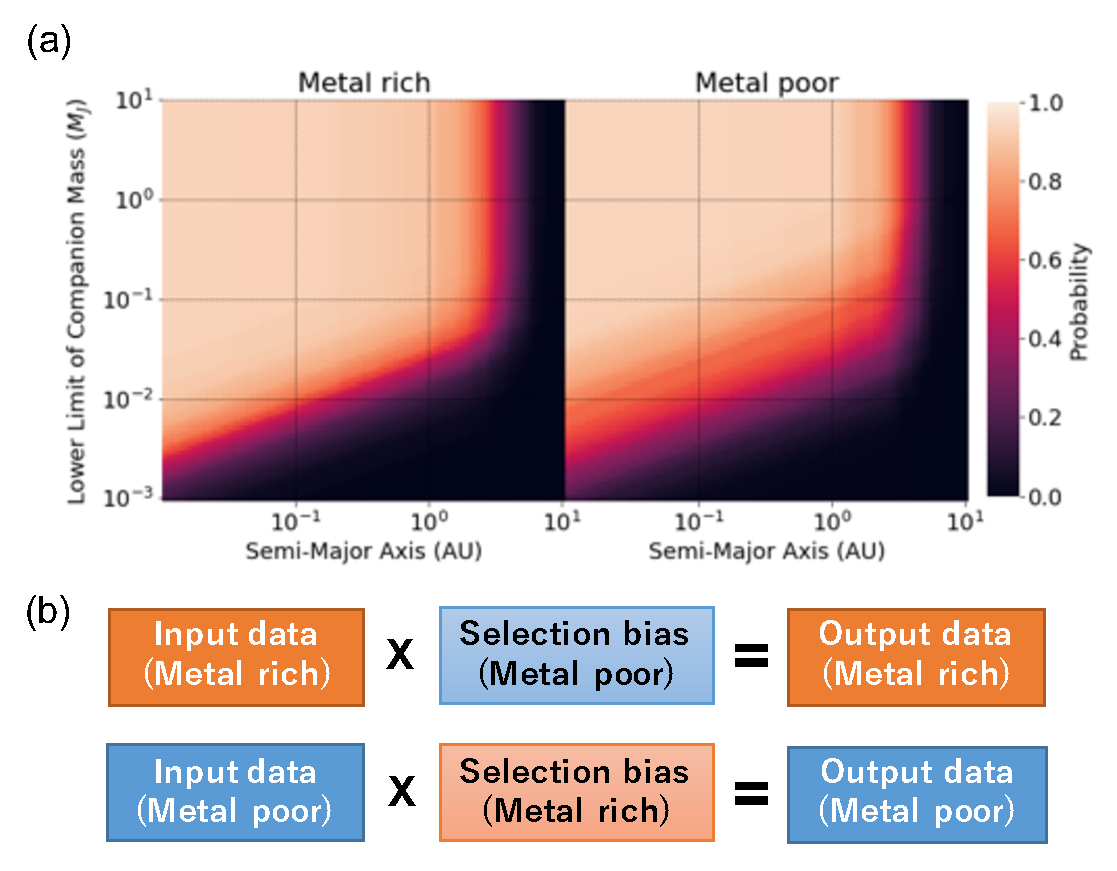
\includegraphics[width=9cm]{../../../Figure/selection_bias.pdf}
\caption{(a) Detectable regions for metal-rich (left) and -poor systems (right). The boundary of metallicity was fixed to 0.0 dex. Each planetary system is observed by the radial velocity measurements with each detection probability. (b) Method for equalizing the two selection biases in two different metallicity regions. The planetary distribution is additionally filtered with the opposite selection bias to remove the different selection biases in the two metallicity regions. \label{fig:bias}}
\end{center}
\end{figure}

First, we determined the boundary of metallicity, which makes the two divided planetary-mass distributions as most different, to verify the possibility of the effect due to the selection biases, and compared the two regions. Changing the metallicity boundary from -0.7 to 0.4 dex, we made the two regions' dataset, and evaluated the planetary-mass distributions with Anderson-Darling (AD) test. Note that we extracted randomly the values of planetary parameters considered their errors, and filtered each sample with any selection biases to remove the calculation bias. Then, the simulations were iterated until the value of boundary was settled. As the result, we found that the best border of metallicity is -0.09 dex. Dividing data with this border, we compared the planetary-mass distributions of both regions. The left of Figure \ref{fig:a_Mp}, (a) shows the relation between semi-major axes and planetary mass, and the right one is the cumulative of planetary mass. AD test for the metal-rich and -poor regions showed that the p-value is $5.6\times10^{-5}$, which can low enough to dismiss the two samples. Thus, we proposed that there is no effect of selection biases for planetary distribution, and exists a difference between the each metallicity region.


\section{Results} \label{sec:results}

In this section, we quantitively show the difference of distributions in metal-rich and -poor regions, and classify the planetary distributions into clusters with Gaussian Mixture Model (GMM). We also show the difference of eccentricity distributions between the classified clusters.


\subsection{Two Regions devided by Metallicity Boundary} \label{subsec:mass}

First, we determined the metallicity boundary by using the method explained in Section ?. Figure \ref{fig:pvalue} shows the p-values calculated by AD test for the distributions of semi-major axis or lower limit of companion mass with converting the boundary of metallicity from -0.7 to 0.4 (dex). We calculated the simulation with 1,000 iteration, which is the enough number of times to settle the each value. The minimum p-values of each parameter were $2.4\times10^{-3}$ and $3.5\times10^{-5}/4.2\times10^{-5}$ at the metallicity boundaries of -0.04 and -0.29/-0.06 (dex), respectively. In this study, we used -0.06 (dex) calculated from the distribution of planetary mass as the best, considering that of the distribution of semi-major axis, and decided to set the boundary of metallicity to -0.05 (dex) that is mean value of each best p-value.

Second, we compared the two regions divided by the optimized boundary of metallicity. Figure \ref{fig:a_Mp} shows that the distributions on the plane of semi-major axis and planetary mass, and the cumulative maps of each parameter. From this figure, we verified the difference between the metal-rich and -poor samples. Thus, we found that there is no effect of the selection bias between the each metallicity region. We also found that planets with short semi-major axis are almost in metal-rich region, which implies that these planets are excited by a dynamical interaction in disks.

\begin{figure}[t]
\begin{center}
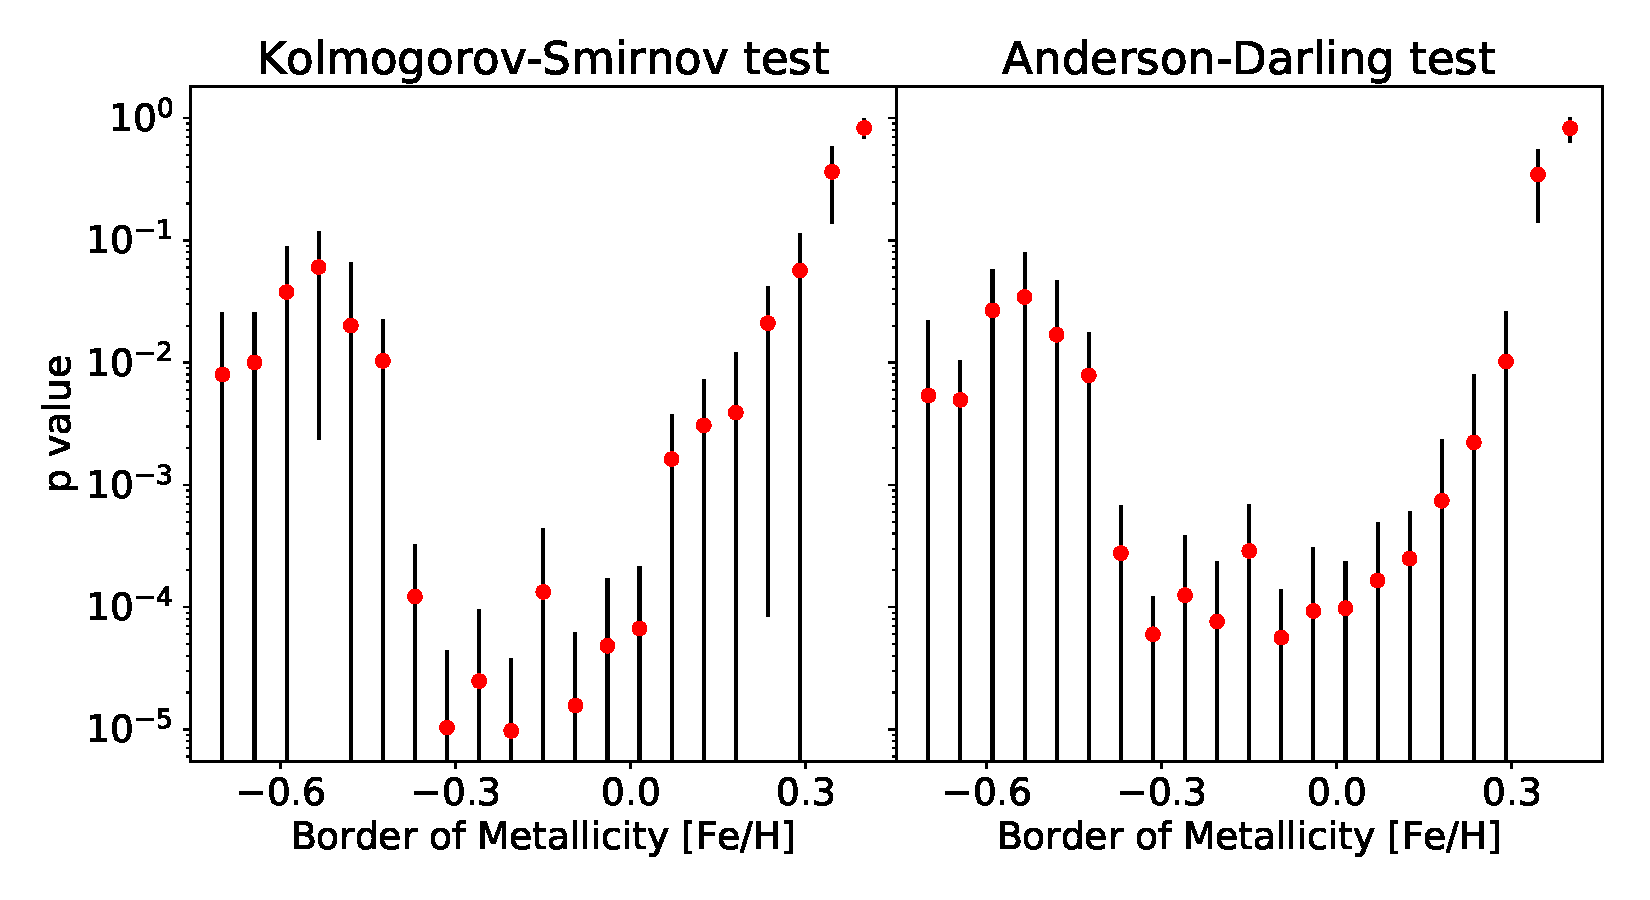
\includegraphics[width=9cm]{../../../Figure/pvalues_plot.pdf}
\caption{P-values of AD test for the samples divided by the changeable boundary of metallicity on semi-major axis (left) and lower limit of companion mass (right). Red points and black vertical bars are p-values and their standard deviations calculated with 1000 iterations. \label{fig:pvalue}}
\end{center}
\end{figure}

\begin{figure}[t]
\begin{center}
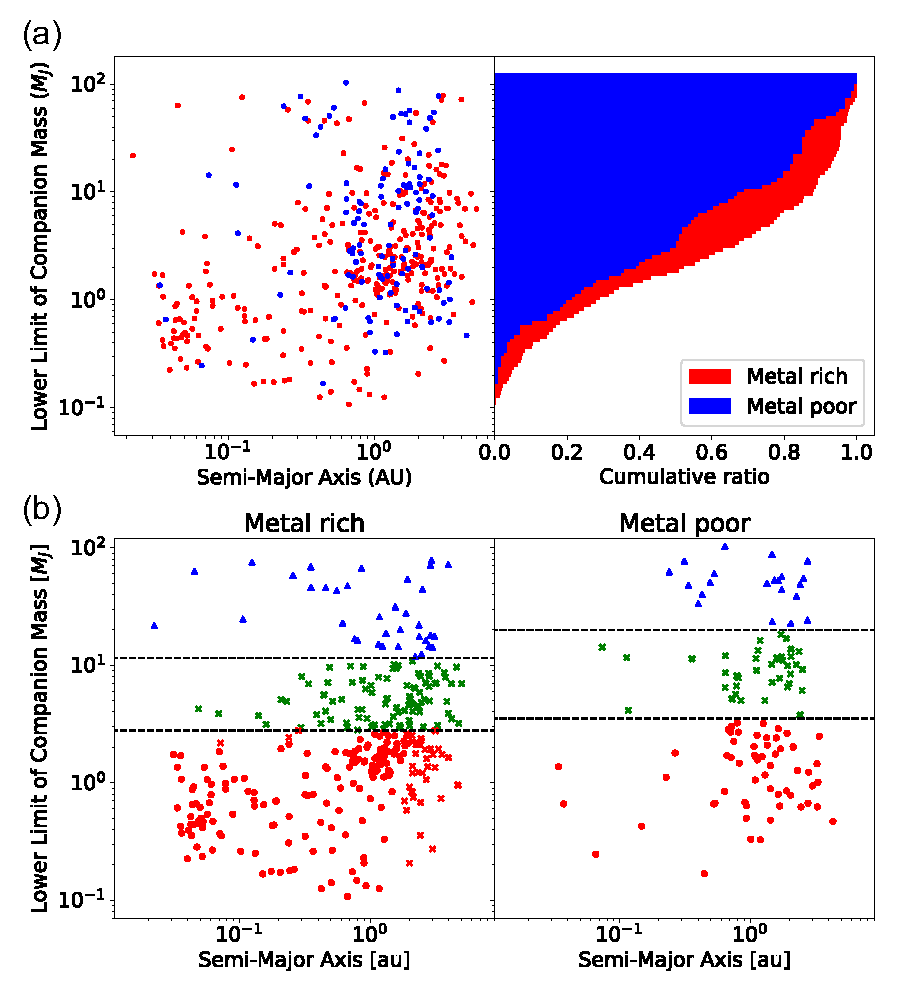
\includegraphics[width=9cm]{../../../Figure/a_Mp.pdf}
\caption{Planetary distributions of the metal-rich and -poor samples (upper left), and cumulative maps of semi-major axis (bottom) and lower limit of companion mass (right). Red and blue points/bins are metal-rich and -poor samples, respectively. \label{fig:a_Mp}}
\end{center}
\end{figure}


\subsection{Three Fields of Planetary Distribution}

We classified the planetary distribution on the star-metallicity and planet-mass plane with a classifier, GMM, which can classify the samples as the number of clusters assumed that each sample extend as a gaussian distribution \citep[e.g.,][]{2017A&A...603A..30S, 2018ApJ...853...37S}. Converting the number of clusters, we evaluated each model with Bayesian Information Criterion (BIC), and found that the best number of clusters for these samples was three, when the BIC score was 3874. Figure \ref{fig:gmm} shows the result of classification of planetary distribution with the best number of clusters. The black horizontal dash lines are the borders of planetary masses dividing the samples into three regions, drawn at 4 and 20 $\rm M_J$. The black vertical dotted lines and gray regions are the means and standard errors of metallicity in each mass field. The mean values are 0.07, -0.01, and -0.13 (dex) in the low-, middle-, and high-mass fields, respectively.

We also verified the eccentricity distributions in both metal-rich and -poor regions, where the planetary masses are divided into three fields. The tops of Figure \ref{fig:e_Mp} are scatter maps of samples on the eccentricity and lower limit of companion mass plane in each metal region after classification of planetary distribution with the mass boundaries obtained from GMM. The bottoms are the cumulative maps of the eccentricity in each region and cluster. The low- and middle-mass fields distribute differently in the metal-rich region. We evaluated the samples of these two fields by AD test, and found that the p-values was $5.0\times10^{-5}$. In contrast, the distribution of the low- and middle-mass fields in the metal-poor region are very similar. This result is consistent with the observational fact that a planet in metal-rich region can be excited by planet-planet and/or planet-disk interaction \citep[e.g.,][]{2013A&A...560A..51A, 2013ApJ...767L..24D}, which causes its eccentricity to grow. On the other hand, the distribution of high-mass fields in each region are almost uniform. This result means that the formation process of the planets over 20 $\rm M_J$ differs from other planets.

\begin{figure}[t]
\begin{center}
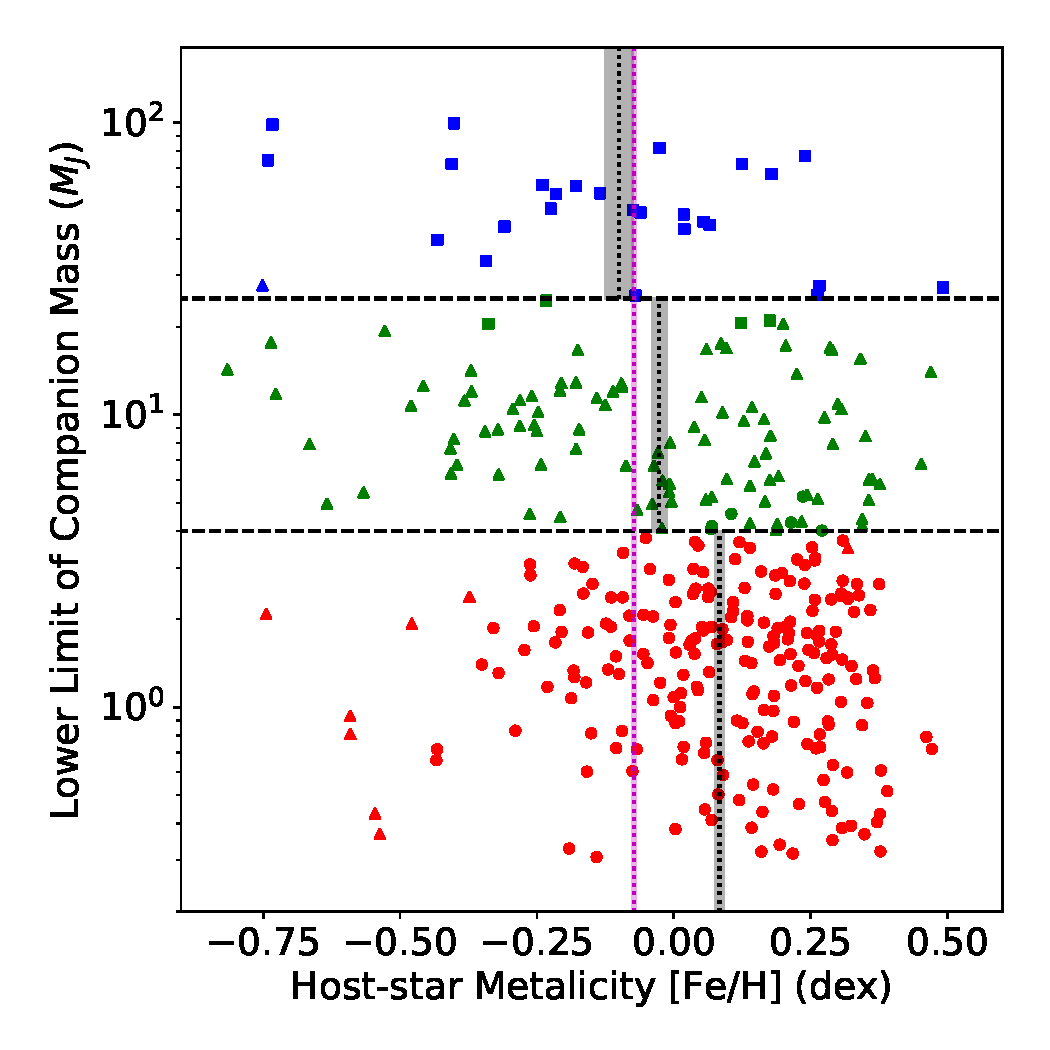
\includegraphics[width=7cm]{../../../Figure/gmm.pdf}
\caption{Distribution classified into three clusters from GMM. The samples of each cluster is described with different markers of square, triangle, and circle. The blue, green, and red points are samples divide into three fields by the mass boundaries (black horizontal lines). The black vertical lines and gray regions are the means and standard errors of metallicity in each field. \label{fig:gmm}}
\end{center}
\end{figure}

\begin{figure}[t]
\begin{center}
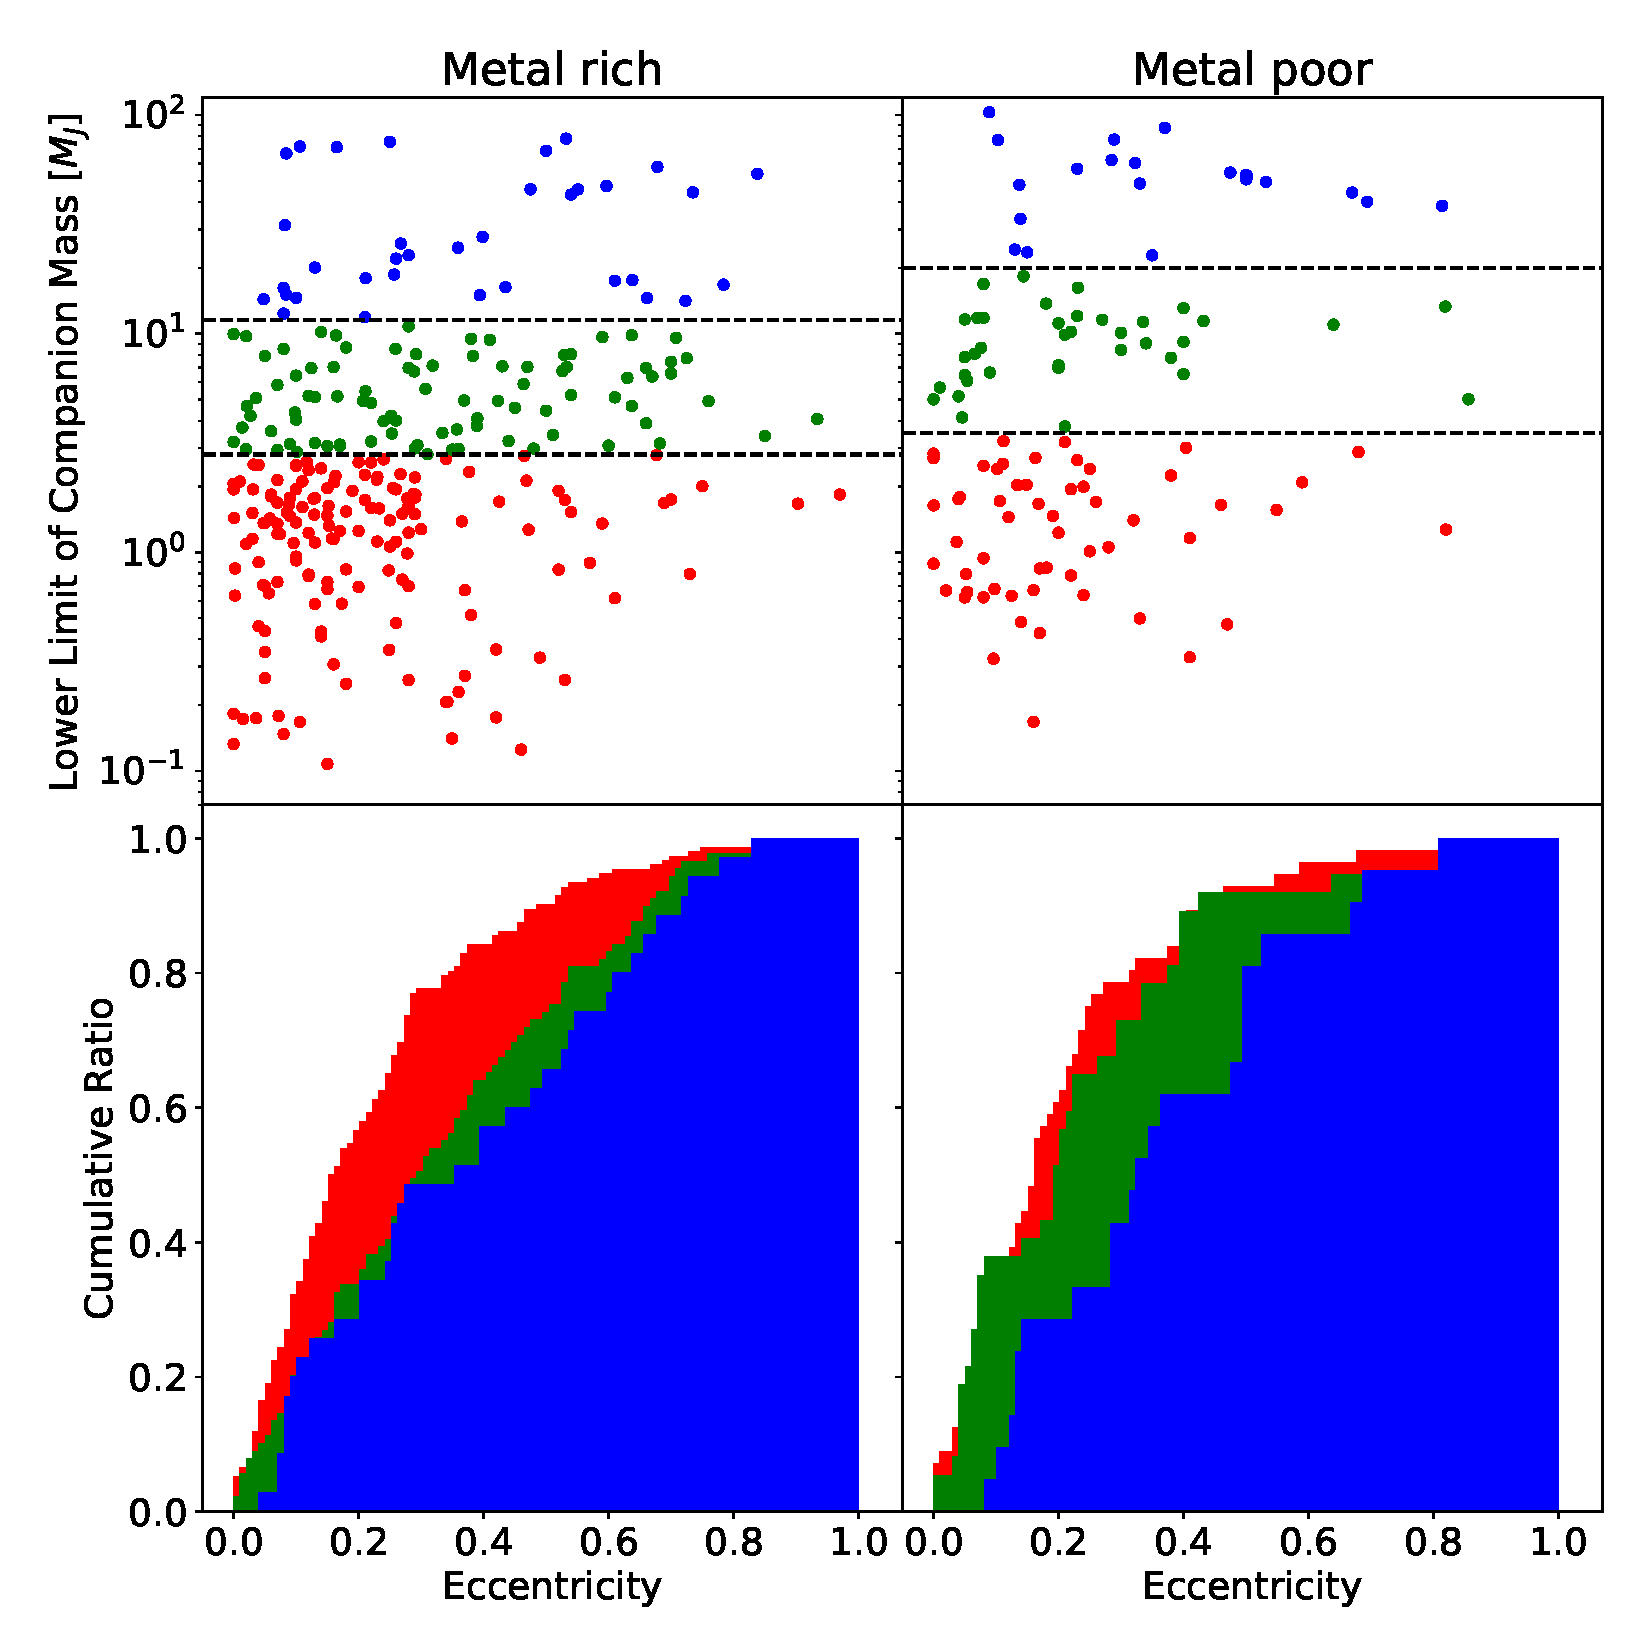
\includegraphics[width=9cm]{../../../Figure/e_Mp_merge.pdf}
\caption{Scatter maps of eccentricities and lower limit of companion masses (top), and cumulative maps of eccentricities (bottom). These colors are the same as those of Figure \ref{fig:gmm}, and corresponding to the top and bottom figures. \label{fig:e_Mp}}
\end{center}
\end{figure}


\section{Discussion}

In this section, we compare the above results of planetary mass and eccentricity distributions with previous studies and verify the relationship. We also discuss the behavior of planetary distributions in the metal-rich and -poor regions, comparing the observed dataset from the simulation of \cite{2012A&A...541A..97M}.


\subsection{?}

In \cite{2012A&A...541A..97M}, planets are formed by classical core accretion model, and the final semi-major axes and planetary masses are determined, based on the simulation included the planetary migration in disks and the disk evolution. From our study, the two observed planetary-mass distributions, which were divided by the metal boundary, had different expanses. Then, we discuss each planetary-formation process, comparing the distribution of observed data with that of simulation data. Figure \ref{fig:simulation} shows that the comparison between the observed data included the selection biases and simulation data cited from \cite{2012A&A...541A..97M}. The simulation data were also filtered by both selection biases of metal-rich and -poor regions to complete the conditions with the observed data. As the result, the distributions of metal rich regions are very consistence, which can explain that most of gas giants in the metal rich region are formed by core accretion. This is also explained by our results shown in Section \ref{subsec:eccentricity} because of below interpretation. The interaction between a gas giant and protoplanetary disk possibly makes the eccentricity of planet grow \citep{2003ApJ...585.1024G, 2006A&A...447..369K}. This interaction is concentrated at discrete Lindblad and corotation resonances, which causes the planet's orbit to migrate and open a gap in the disk as the planet mass is large enough. If the viscous coefficient equals to $10^{-5}$, the planet with circular orbit changes to eccentric orbit as the planetary mass is over 3 $\rm M_J$. The more massive planets make their eccentricity higher until the maximum value 0.25. On the other hand, if a planetary system has two gas giants, the outer planet may prolong the orbital period of the inner planet. These planets' eccentricities grow up in rough inverse proportion to their masses by this orbital interaction \citep{2002ApJ...564L.105C}. From the verification of simulation \citep{2013ApJ...775...42I}, gas giants and rocky/icy planets emerge, migrate, and undergo dynamical instability in a relatively massive disk, and the perturbation between planets causes orbital crossing, eccentricity excitation, and planetary ejection. Therefore, gas giants formed through core accretion tend to have high eccentricities, which is consistent to our results of eccentricity distribution.

In contrast, the distributions of metal poor regions between the observed data and the simulation data are different. This means that the planetary formation process in metal poor disks differs from in metal rich disks: the planetary formation in metal poor region cannot be explained by only core accretion. On the other hand, the eccentricity of gas giant formed via disk instability ranges from 0 to 0.35 in initial stage, and decreases as the planet mass increases \citep{2011ApJ...731...74B}. Note that the range of semi-major axis is $30\sim70$ au. This trend can be also seen slightly in the metal poor region of Figure \ref{fig:e_Mp}. However, because it is not clear, there possibly exists other formation processes included core accretion in metal poor regions.

\begin{figure}[t]
\begin{center}
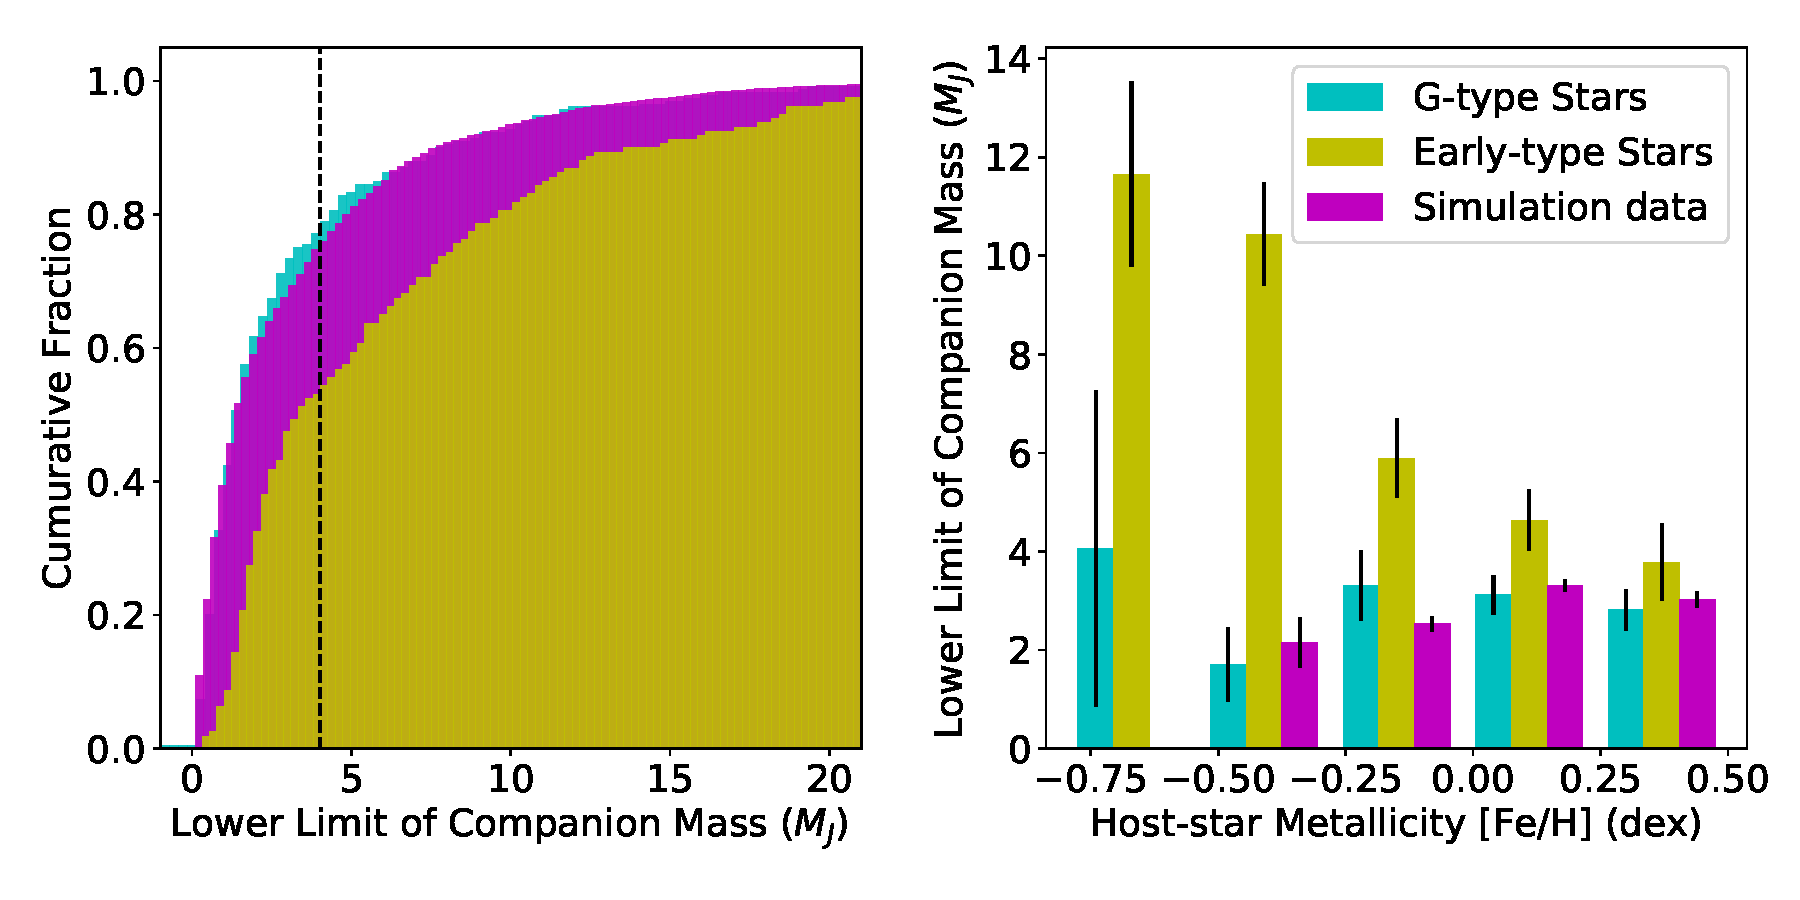
\includegraphics[width=9cm]{../../../Figure/simulation.pdf}
\caption{Comparison of planetary distributions between the observed data (red and blue points) and simulation data (yellow and cyan points) in the metal-rich region (upper left) and the metal-poor region (lower left), and the cumulative maps of planetary masses in the metal-rich region (upper right) and the metal-poor region (lower right). \label{fig:simulation}}
\end{center}
\end{figure}


\subsection{?}

According to previous studies, the planetary distributions are divided into two regions. Host stars over 4 $M_J$ tend to be more metal poor and massive, but below this value show the well-known metallicity-giant planet frequency correlation \citep{2017A&A...603A..30S}. In addition, planets formed through core accretion have upper bound of mass, which equals around 10 $M_J$, and planets over this value likely formed through gravitational disk instability \citep{2018ApJ...853...37S}.  However, we show that the planetary distribution has multiple regions depending on planetary mass and disk metallicity. Figure \ref{fig:metal_Mp} shows that the planetary distribution used in this study. The colors of red and blue mean the planets in metal rich and poor regions, respectively. The markers describe the different ranges of planet mass, which divided with mass boundary determined by the classification in Section \ref{subsec:mass}. 

\textcolor{green}{According to previous studies, the distribution of gas-giant masses can be divided into two regions by the border of 4 $\rm M_J$ with metallicity bias, which insists that the planetary-formation processes in each region are different \citep[e.g.,][]{2017A&A...603A..30S}. In contrast, the boundaries were drawn at 4 and 20 $\rm M_J$ from our result, which the former is consistent with the previous studies. The latter indicates the border between the gas giants and brawn dwarfs.}

\begin{figure*}[t]
\begin{center}
\includegraphics[width=15cm]{../../../Figure/metal_Mp.pdf}
\caption{\label{fig:metal_Mp}}
\end{center}
\end{figure*}


\acknowledgments


\vspace{5mm}


\begin{thebibliography}{}

\bibitem[Adibekyan et al.(2013)]{2013A&A...560A..51A} Adibekyan, V.~Z., Figueira, P., Santos, N.~C., et al.\ 2013, \aap, 560, A51
\bibitem[Boss(1997)]{1997Sci...276.1836B} Boss, A.~P.\ 1997, Science, 276, 1836
\bibitem[Boss(2002)]{2002ApJ...567L.149B} Boss, A.~P.\ 2002, \apjl, 567, L149
\bibitem[Boss(2011)]{2011ApJ...731...74B} Boss, A.~P.\ 2011, \apj, 731, 74
\bibitem[Buchhave et al.(2012)]{2012Natur.486..375B} Buchhave, L.~A., Latham, D.~W., Johansen, A., et al.\ 2012, \nat, 486, 375
\bibitem[Cai et al.(2006)]{2006ApJ...636L.149C} Cai, K., Durisen, R.~H., Michael, S., et al.\ 2006, \apjl, 636, L149
\bibitem[Casagrande et al.(2011)]{2011A&A...530A.138C} Casagrande, L., Sch{\"o}nrich, R., Asplund, M., et al.\ 2011, \aap, 530, A138
\bibitem[Chiang et al.(2002)]{2002ApJ...564L.105C} Chiang, E.~I., Fischer, D., \& Thommes, E.\ 2002, \apjl, 564, L105
\bibitem[Dawson \& Murray-Clay(2013)]{2013ApJ...767L..24D} Dawson, R.~I., \& Murray-Clay, R.~A.\ 2013, \apjl, 767, L24
\bibitem[Dupuy \& Liu(2011)]{2011ApJ...733..122D} Dupuy, T.~J., \& Liu, M.~C.\ 2011, \apj, 733, 122
\bibitem[Durisen et al.(2007)]{2007Arizona} Durisen, R. H., Reipurth, V. Jewitt, Keil, K., et al.\ 2007, Univ. of Arizona Press, Tucson 951, 607-622
\bibitem[Fischer \& Valenti(2005)]{2005ApJ...622.1102F} Fischer, D.~A., \& Valenti, J.\ 2005, \apj, 622, 1102
\bibitem[Girardi et al.(2000)]{2000A&AS..141..371G} Girardi, L., Bressan, A., Bertelli, G., \& Chiosi, C.\ 2000, \aaps, 141, 371
\bibitem[Goldreich \& Sari(2003)]{2003ApJ...585.1024G} Goldreich, P., \& Sari, R.\ 2003, \apj, 585, 1024
\bibitem[Hayashi et al.(1985)]{1985prpl.conf.1100H} Hayashi, C., Nakazawa, K., \& Nakagawa, Y.\ 1985, Protostars and Planets II, 1100
\bibitem[Hidalgo et al.(2018)]{2018ApJ...856..125H} Hidalgo, S.~L., Pietrinferni, A., Cassisi, S., et al.\ 2018, \apj, 856, 125
\bibitem[Ida \& Lin($2004_a$)]{2004ApJ...604..388I} Ida, S., \& Lin, D.~N.~C.\ 2004, \apj, 604, 388
\bibitem[Ida \& Lin($2004_b$)]{2004ApJ...616..567I} Ida, S., \& Lin, D.~N.~C.\ 2004, \apj, 616, 567
\bibitem[Ida et al.(2013)]{2013ApJ...775...42I} Ida, S., Lin, D.~N.~C., \& Nagasawa, M.\ 2013, \apj, 775, 42
\bibitem[Kley \& Dirksen(2006)]{2006A&A...447..369K} Kley, W., \& Dirksen, G.\ 2006, \aap, 447, 369
\bibitem[Kuiper(1951)]{1951PNAS...37....1K} Kuiper, G.~P.\ 1951, Proceedings of the National Academy of Science, 37, 1
\bibitem[Lee et al.(2012)]{2012MNRAS.424.2832L} Lee, K.~J., Guillemot, L., Yue, Y.~L., Kramer, M., \& Champion, D.~J.\ 2012, \mnras, 424, 2832
\bibitem[Ma \& Ge(2014)]{2014MNRAS.439.2781M} Ma, B., \& Ge, J.\ 2014, \mnras, 439, 2781
\bibitem[Matsuo et al.(2007)]{2007ApJ...662.1282M} Matsuo, T., Shibai, H., Ootsubo, T., \& Tamura, M.\ 2007, \apj, 662, 1282
\bibitem[Mayor \& Queloz(1995)]{1995Natur.378..355M} Mayor, M., \& Queloz, D.\ 1995, \nat, 378, 355
\bibitem[Mayer et al.(2002)]{2002Sci...298.1756M} Mayer, L., Quinn, T., Wadsley, J., \& Stadel, J.\ 2002, Science, 298, 1756
\bibitem[Mayer et al.(2007)]{2007ApJ...661L..77M} Mayer, L., Lufkin, G., Quinn, T., \& Wadsley, J.\ 2007, \apjl, 661, L77
\bibitem[Mayor et al.(2011)]{2011arXiv1109.2497M} Mayor, M., Marmier, M., Lovis, C., et al.\ 2011, arXiv:1109.2497
\bibitem[Mizuno(1980)]{1980PThPh..64..544M} Mizuno, H.\ 1980, Progress of Theoretical Physics, 64, 544
\bibitem[Mordasini et al.(2009)]{2009A&A...501.1161M} Mordasini, C., Alibert, Y., Benz, W., \& Naef, D.\ 2009, \aap, 501, 1161
\bibitem[Mordasini et al.(2012)]{2012A&A...541A..97M} Mordasini, C., Alibert, Y., Benz, W., Klahr, H., \& Henning, T.\ 2012, \aap, 541, A97
\bibitem[Perri \& Cameron(1974)]{1974Icar...22..416P} Perri, F., \& Cameron, A.~G.~W.\ 1974, \icarus, 22, 416
\bibitem[Pollack et al.(1996)]{1996Icar..124...62P} Pollack, J.~B., Hubickyj, O., Bodenheimer, P., et al.\ 1996, \icarus, 124, 62
\bibitem[Ribas \& Miralda-Escud{\'e}(2007)]{2007A&A...464..779R} Ribas, I., \& Miralda-Escud{\'e}, J.\ 2007, \aap, 464, 779
\bibitem[Santos et al.(2003)]{2003A&A...398..363S} Santos, N.~C., Israelian, G., Mayor, M., Rebolo, R., \& Udry, S.\ 2003, \aap, 398, 363
\bibitem[Santos et al.(2017)]{2017A&A...603A..30S} Santos, N.~C., Adibekyan, V., Figueira, P., et al.\ 2017, \aap, 603, A30
\bibitem[Schlaufman(2018)]{2018ApJ...853...37S} Schlaufman, K.~C.\ 2018, \apj, 853, 37
\bibitem[Schneider et al.(2011)]{2011A&A...532A..79S} Schneider, J., Dedieu, C., Le Sidaner, P., Savalle, R., \& Zolotukhin, I.\ 2011, \aap, 532, A79
\bibitem[Sousa et al.(2018)]{2018A&A...620A..58S} Sousa, S.~G., Adibekyan, V., Delgado-Mena, E., et al.\ 2018, \aap, 620, A58
\bibitem[Tanigawa \& Tanaka(2016)]{2016ApJ...823...48T} Tanigawa, T., \& Tanaka, H.\ 2016, \apj, 823, 48
\bibitem[Torres et al.(2008)]{2008ApJ...677.1324T} Torres, G., Winn, J.~N., \& Holman, M.~J.\ 2008, \apj, 677, 1324
\bibitem[Wang \& Fischer(2015)]{2015AJ....149...14W} Wang, J., \& Fischer, D.~A.\ 2015, \aj, 149, 14
\bibitem[Weiss et al.(2013)]{2013ApJ...768...14W} Weiss, L.~M., Marcy, G.~W., Rowe, J.~F., et al.\ 2013, \apj, 768, 14

\end{thebibliography}

%\appendix

\end{CJK*}
\end{document}
